% ============================================================
%  Chapter 2 – Heuristics for the Vehicle Routing Problem
%  Self-contained Beamer slides (reader-friendly lecture notes)
%  Source: "Nature Inspired Optimisation for Delivery Problems" (2022)
% ============================================================
\documentclass[aspectratio=169,10pt]{beamer}

\usetheme{Madrid}
\usecolortheme{seahorse}
\setbeamertemplate{footline}[frame number]
\setbeamertemplate{navigation symbols}{}

% ── Packages ────────────────────────────────────────────────
\usepackage{amsmath,amssymb}
\usepackage{graphicx}
\usepackage{listings}
\usepackage{xcolor}
\usepackage{booktabs}
\usepackage{array}
\usepackage{microtype}
\usepackage{tikz}
\usetikzlibrary{arrows.meta,shapes.geometric,positioning,fit,backgrounds}

\graphicspath{{figures/}}

% ── Listings style ──────────────────────────────────────────
\definecolor{codebg}{rgb}{0.97,0.97,0.97}
\definecolor{codegreen}{rgb}{0.0,0.5,0.2}
\definecolor{codepurple}{rgb}{0.4,0.0,0.6}
\definecolor{codekw}{rgb}{0.1,0.1,0.7}
\lstset{
  language=Python,
  basicstyle=\ttfamily\scriptsize,
  numbers=left,
  numberstyle=\tiny\color{gray},
  frame=single,
  backgroundcolor=\color{codebg},
  commentstyle=\color{codegreen}\itshape,
  keywordstyle=\color{codekw}\bfseries,
  stringstyle=\color{codepurple},
  showstringspaces=false,
  breaklines=true,
  tabsize=4,
  xleftmargin=1.5em,
  framexleftmargin=1.5em,
  captionpos=b,
}

% ── Meta ────────────────────────────────────────────────────
\title[VRP Heuristics]{Chapter 2: Heuristics for the Vehicle Routing Problem}
\subtitle{Nature Inspired Optimisation for Delivery Problems (2022)}
\author{Lecture Slides}
\date{}

% ============================================================
\begin{document}
% ============================================================

% ── Title ───────────────────────────────────────────────────
\begin{frame}
  \titlepage
\end{frame}

% ── Overview ────────────────────────────────────────────────
\begin{frame}[allowframebreaks]{Chapter Overview}

  This chapter introduces the \textbf{Vehicle Routing Problem (VRP)} --- one of
  the most practically important combinatorial optimisation problems, arising
  whenever goods must be delivered from a central warehouse to a dispersed set
  of customers.  Unlike the Travelling Salesman Problem (TSP) studied in
  Chapter~1, the VRP requires planning \emph{multiple} routes simultaneously,
  subject to the constraint that each vehicle can carry only a limited load.

  \bigskip
  The chapter is organised as follows:

  \begin{itemize}
    \item \textbf{Section 2.1} defines the Capacitated Vehicle Routing Problem
      (CVRP) precisely, introducing the concepts of routes, demands, and vehicle
      capacity.
    \item \textbf{Section 2.2} introduces three algorithms for solving the CVRP:
      the \emph{Grand Tour} construction, the \emph{Clarke--Wright savings}
      algorithm, and discusses the 2-opt local-search improvement.
    \item \textbf{Section 2.3} presents a Java implementation (with Python
      equivalents) and describes the class structure.
    \item \textbf{Section 2.4} benchmarks both heuristics on the standard
      Augerat problem sets and compares them with branch-and-cut.
    \item \textbf{Section 2.5} draws conclusions and motivates the need for more
      powerful metaheuristics.
  \end{itemize}

  \begin{alertblock}{Key Takeaway}
    Simple heuristics such as Clarke--Wright are fast and easy to implement,
    but produce solutions that are 5--27\% longer than optimal.  More
    sophisticated nature-inspired techniques (introduced in later chapters)
    are needed to close this gap.
  \end{alertblock}

\end{frame}

% ============================================================
%  SECTION 2.1 – THE CVRP
% ============================================================
\section{2.1 The Vehicle Routing Problem}

\begin{frame}[allowframebreaks]{Motivation: From TSP to VRP}

  The \textbf{Travelling Salesman Problem (TSP)} asks for the shortest
  \emph{single} tour that visits every city exactly once.  In reality, however,
  a delivery company rarely has just one vehicle.  Instead, it operates a
  \emph{fleet}, and each vehicle has a maximum weight or volume it can carry.
  The question then becomes: how should we divide customers among vehicles,
  and in what order should each vehicle visit its assigned customers?

  \bigskip
  This is the \textbf{Vehicle Routing Problem (VRP)}, first studied by
  Dantzig and Ramser in 1959.  The VRP generalises the TSP: every VRP
  solution consists of a set of TSP-like tours (called \emph{routes}), each
  starting and ending at a central \textbf{depot}.

  \bigskip
  \begin{block}{The Capacitated VRP (CVRP) --- Informal Statement}
    Given a depot and a set of customers, each with a known demand, assign
    customers to vehicles and plan a route for each vehicle such that:
    \begin{enumerate}
      \item every customer is visited exactly once,
      \item the total demand on any route does not exceed the vehicle capacity
        $Q$ (Q, the maximum load a vehicle can carry),
      \item the number of vehicles used is minimised,
      \item the total distance driven by all vehicles is minimised.
    \end{enumerate}
  \end{block}

  \medskip
  The two objectives (minimise vehicles, minimise distance) are often treated
  lexicographically: first minimise vehicles, then minimise distance.

  \framebreak

  \begin{block}{Running Example: ACE Doughnuts}
    Throughout this chapter we use a concrete motivating scenario.  ACE
    Doughnuts operates a factory that bakes doughnuts to order.  Customers
    place orders the previous day.  The factory owns a fleet of vans, each
    capable of carrying $capacity$ doughnuts.  Each day a delivery plan must
    be computed satisfying:
    \begin{itemize}
      \item No van carries more than $capacity$ doughnuts.
      \item Every customer receives exactly the number they ordered.
      \item The number of vans used is minimised.
      \item The total distance driven by all vans is minimised.
    \end{itemize}
  \end{block}

  This scenario maps directly onto the CVRP: customers correspond to delivery
  addresses, demands correspond to order sizes, the depot is the factory, and
  vehicle capacity is the maximum load per van.

\end{frame}

% ── CVRP formal definition ──────────────────────────────────
\begin{frame}[allowframebreaks]{Formal Definition of the CVRP}

  We now define the CVRP precisely.  The problem is specified by a graph
  whose nodes represent the depot and the customers.

  \bigskip
  \begin{block}{Notation}
    \begin{tabular}{@{}ll}
      $n$           & number of customers \\
      $d$           & depot (the start/end location of all routes) \\
      $c_i$         & customer $i$, for $i = 1, \ldots, n$ \\
      $\delta_i$    & demand (delta, $\delta$) of customer $i$: the
                       quantity that must be delivered to $c_i$ \\
      $Q$           & vehicle capacity: the maximum total demand a
                       single vehicle can service on one route \\
      $\mathrm{dist}(a, b)$ & Euclidean distance between nodes $a$ and $b$ \\
    \end{tabular}
  \end{block}

  \medskip
  Here $\delta_i$ (delta) is the Greek letter commonly used for ``difference''
  or ``quantity''; in this context it represents how many units customer $i$
  needs.  The symbol $Q$ (for Quantity/Capacity) is the hard upper limit
  on how much any single vehicle can carry.

  \framebreak

  \begin{block}{A CVRP Solution}
    A \textbf{solution} is a set of routes
    $R = \{r_1, r_2, \ldots, r_k\}$, where $k$ is the number of vehicles.
    Each route $r_j$ is an ordered list of customers:
    \[
      r_j = (d,\; c_{j_1},\; c_{j_2},\; \ldots,\; c_{j_{m_j}},\; d)
    \]
    meaning the vehicle departs from the depot $d$, visits customers
    $c_{j_1}, c_{j_2}, \ldots$ in that order, and returns to $d$.
  \end{block}

  \begin{block}{Feasibility Constraints}
    A solution is \textbf{feasible} if and only if:
    \begin{enumerate}
      \item \textbf{Coverage}: every customer $c_i$ appears in exactly one route.
      \item \textbf{Capacity}: for every route $r_j$,
        \[
          \sum_{i \in r_j} \delta_i \;\leq\; Q
        \]
        That is: the sum ($\Sigma$, sigma, meaning ``add up'') of demands of all
        customers in route $r_j$ does not exceed the vehicle capacity $Q$.
    \end{enumerate}
  \end{block}

  The capacity constraint is the key feature distinguishing CVRP from TSP.
  Think of it as a weight limit: once a van is full, it cannot take on more
  parcels --- it must return to the depot first.

  \framebreak

  \begin{block}{Objective Function}
    The total cost of a solution (total distance driven by all vehicles) is:
    \[
      \text{TotalDist}(R) \;=\;
      \sum_{j=1}^{k} \mathrm{dist}(r_j)
    \]
    where $\mathrm{dist}(r_j)$ is the total distance of route $r_j$, computed
    as the sum of consecutive edge lengths:
    \[
      \mathrm{dist}(r_j) =
      \mathrm{dist}(d, c_{j_1})
      + \sum_{l=1}^{m_j - 1} \mathrm{dist}(c_{j_l}, c_{j_{l+1}})
      + \mathrm{dist}(c_{j_{m_j}}, d)
    \]
  \end{block}

  \begin{alertblock}{How to Read This Formula}
    The outer sum adds up the distance of each individual route.  For a
    single route, the distance is: depot to first customer, then customer to
    customer along the route, then last customer back to depot.  Doubling the
    number of customers on a route roughly doubles the distance driven for
    that route --- but the capacity $Q$ acts as a ceiling that forces the route
    to be split before it grows too long.
  \end{alertblock}

  \framebreak

  \begin{block}{Minimum Number of Vehicles}
    A lower bound on the number of vehicles required is:
    \[
      k_{\min} = \left\lceil \frac{\sum_{i=1}^{n} \delta_i}{Q} \right\rceil
    \]
    Here $\lceil \cdot \rceil$ (ceiling function) rounds up to the nearest
    integer, because we cannot use a fractional vehicle.
    $\sum_{i=1}^{n} \delta_i$ is the total demand across all customers.
  \end{block}

  \begin{exampleblock}{Worked Example: 8-Customer Instance}
    The book's example has 8 customers with demands
    $\delta_1=5,\;\delta_2=4,\;\delta_3=6,\;\delta_4=5,\;\delta_5=2,\;\delta_6=3,\;\delta_7=3,\;\delta_8=4$
    and vehicle capacity $Q=10$.

    Total demand $= 5+4+6+5+2+3+3+4 = 32$.

    \medskip
    $k_{\min} = \lceil 32/10 \rceil = \lceil 3.2 \rceil = 4$ vehicles.

    \medskip
    So at least 4 vehicles are needed.  The solution shown in the figure below
    achieves exactly 4 routes and is therefore optimal in terms of vehicle count.
  \end{exampleblock}

\end{frame}

% ── CVRP figure ─────────────────────────────────────────────
\begin{frame}[allowframebreaks]{CVRP Example: 8 Customers, 4 Routes}

  The figure below shows a valid solution to the small CVRP instance.  The
  depot is at the centre.  Each customer node is labelled with its demand $d$.
  Four coloured routes depart from and return to the depot, each respecting
  the capacity constraint $Q = 10$.

  \begin{center}
    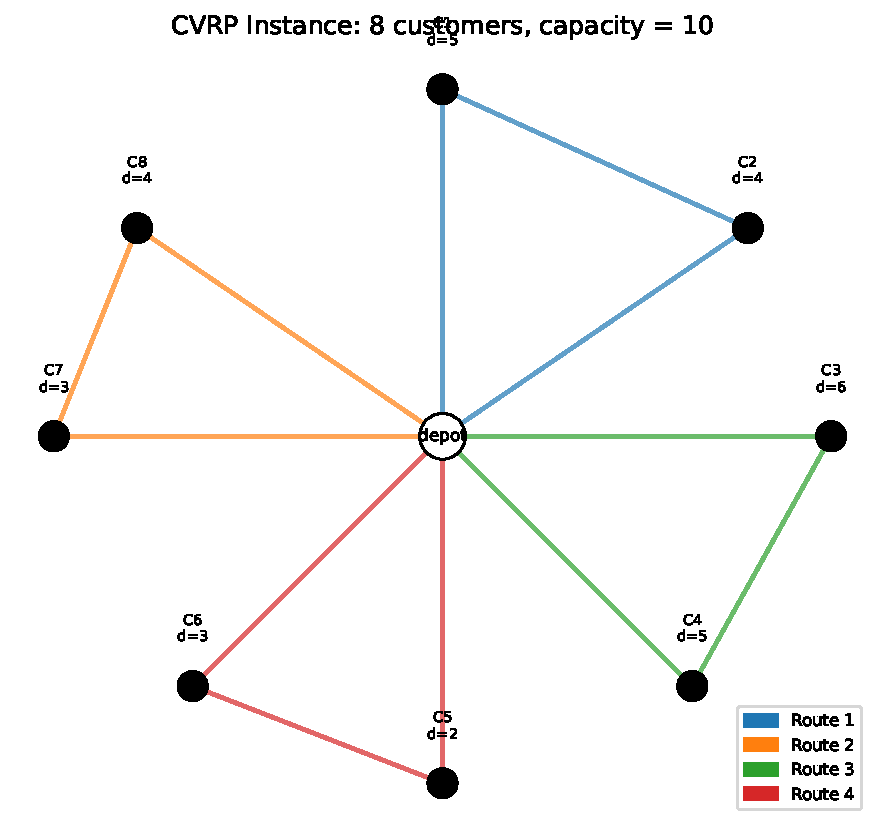
\includegraphics[width=0.55\textwidth]{fig_cvrp_layout.pdf}
  \end{center}

  \medskip
  \textbf{Reading the figure.}  Trace each coloured arc from the depot outward
  to one or more customers and back.  Notice that no route carries more than
  10 units of demand in total: for example, Route~1 visits C1 (demand~5) and
  C2 (demand~4), giving a combined load of 9, which is safely below the
  capacity limit.

  \begin{alertblock}{Two Types of Decision}
    Solving a VRP requires making two interleaved decisions:
    (1)~\textbf{Allocation} --- which customers should be grouped together on
    the same vehicle; and
    (2)~\textbf{Sequencing} --- within a group, in what order should the
    vehicle visit them?  Both decisions jointly determine the total distance.
  \end{alertblock}

\end{frame}

% ── Problem instances ────────────────────────────────────────
\begin{frame}[allowframebreaks]{Benchmark Problem Instances: Augerat Sets}

  To evaluate algorithm performance, researchers use \emph{benchmark instances}
  --- problem instances whose optimal (or best-known) solution is already known,
  so that any new algorithm can be compared against it fairly.

  \bigskip
  This chapter uses the \textbf{Augerat (1995) benchmark}, a widely-used
  collection of 60 CVRP instances grouped into three sets:

  \begin{description}
    \item[Set A] Random instances.  Customers are placed at uniformly random
      positions over a square region.
    \item[Set B] Clustered instances.  Customers tend to group together in
      geographic clusters, which often makes routing easier.
    \item[Set P] Literature-based instances.  These come from earlier published
      VRP research and have varied structure.
  \end{description}

  \medskip
  The number of customer visits $n$ ranges from 15 to 100, with an average
  of 51.  Some instances have a known \emph{optimal} solution (found by branch
  and cut); others only have a \emph{best-known} solution.

  \framebreak

  The figure below shows one representative instance from each set.  The red
  square is the depot; black dots are customer locations.

  \begin{center}
    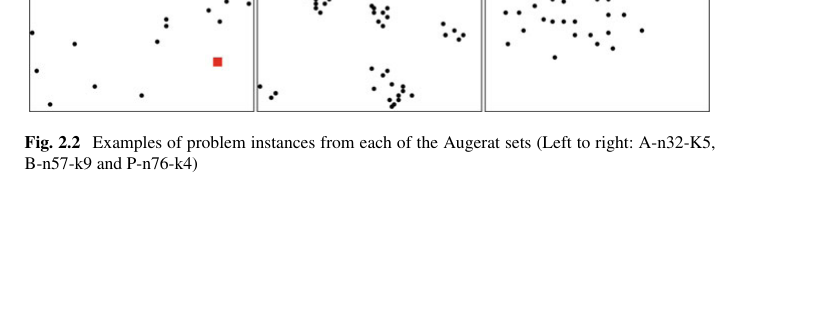
\includegraphics[width=0.85\textwidth]{fig_problem_instances.png}
  \end{center}

  \medskip
  Visually, Set~A instances look like scattered points (no structure), while
  Set~B instances show obvious clusters.  Set~P instances have mixed structure
  inherited from their original authors.

  \begin{alertblock}{Why Benchmarks Matter}
    Without a common benchmark, it is impossible to compare two algorithms
    objectively.  The Augerat set provides the ``ground truth'' against which
    the Grand Tour and Clarke--Wright solvers are evaluated in Section~2.4.
  \end{alertblock}

\end{frame}

% ============================================================
%  SECTION 2.2 – SOLVING THE CVRP
% ============================================================
\section{2.2 Solving the CVRP}

\begin{frame}[allowframebreaks]{Overview of Solution Approaches}

  The CVRP is \textbf{NP-hard}: no polynomial-time algorithm is known to find
  the optimal solution in general.  For practical problem sizes (tens to
  hundreds of customers), we therefore turn to \textbf{heuristics} ---
  algorithms that find good (but not necessarily optimal) solutions in
  reasonable time.

  \bigskip
  This section covers two construction heuristics:
  \begin{enumerate}
    \item The \textbf{Grand Tour} heuristic: build a TSP tour over all customers
      first, then split it into capacity-feasible sub-tours.
    \item The \textbf{Clarke--Wright Savings Algorithm}: start with the worst
      possible solution (one vehicle per customer) and iteratively merge routes
      whenever doing so saves distance.
  \end{enumerate}

  Both produce \emph{feasible} solutions quickly, but with different quality.
  Neither guarantees optimality.

\end{frame}

% ── Grand Tour ──────────────────────────────────────────────
\begin{frame}[allowframebreaks]{The Grand Tour Heuristic}

  The Grand Tour approach is conceptually the simplest way to build a CVRP
  solution.  The key idea is: \textit{first ignore the capacity constraint and
  solve an easier problem (the TSP), then enforce the constraint by splitting
  the single big tour into smaller feasible routes.}

  \bigskip
  \textbf{Step 1 --- Solve a TSP.}  Treat all customers and the depot as
  cities in a TSP.  Use any TSP solver (for example, the Nearest-Neighbour
  heuristic from Chapter~1) to find a tour that visits every customer once
  and returns to the depot.  This produces a single, potentially very long
  route:
  \[
    d \;\to\; c_1 \;\to\; c_2 \;\to\; c_3 \;\to\; \cdots \;\to\; c_n \;\to\; d
  \]

  \textbf{Step 2 --- Split the Grand Tour into sub-tours.}  Walk along the
  Grand Tour from the depot.  Keep adding customers to the current sub-tour
  as long as the cumulative demand does not exceed the vehicle capacity $Q$.
  The moment adding the next customer would exceed $Q$, close the current
  sub-tour (return to depot), open a new one, and continue.

  \framebreak

  \begin{exampleblock}{Worked Example: Splitting the Grand Tour}
    Grand Tour order: $d \to C_1 \to C_2 \to C_3 \to C_4 \to C_5 \to C_6 \to C_7 \to C_8 \to d$

    \medskip
    Demands: $C_1{=}5,\; C_2{=}4,\; C_3{=}6,\; C_4{=}5,\; C_5{=}2,\; C_6{=}3,\; C_7{=}3,\; C_8{=}4$.
    Capacity $Q=10$.

    \medskip
    \begin{tabular}{lll}
      \toprule
      Step & Action & Cumulative demand \\
      \midrule
      1 & Start new route, add $C_1$ & 5 \\
      2 & Add $C_2$: $5+4=9 \leq 10$ & 9 \\
      3 & Try $C_3$: $9+6=15 > 10$ \textbf{--- exceed capacity!} & --- \\
        & Close route: $d \to C_1 \to C_2 \to d$ & \\
      4 & New route, add $C_3$ & 6 \\
      5 & Try $C_4$: $6+5=11 > 10$ \textbf{--- exceed capacity!} & --- \\
        & Close route: $d \to C_3 \to d$ & \\
      6 & New route, add $C_4$, $C_5$, $C_6$: $5+2+3=10 \leq 10$ & 10 \\
      7 & Try $C_7$: $10+3=13 > 10$ \textbf{--- close route} & --- \\
        & Close route: $d \to C_4 \to C_5 \to C_6 \to d$ & \\
      8 & New route, add $C_7$, $C_8$: $3+4=7 \leq 10$ & 7 \\
        & End of tour: close final route & \\
      \bottomrule
    \end{tabular}

    \medskip
    Result: 4 routes, matching the minimum vehicle count.
  \end{exampleblock}

  \framebreak

  \begin{center}
    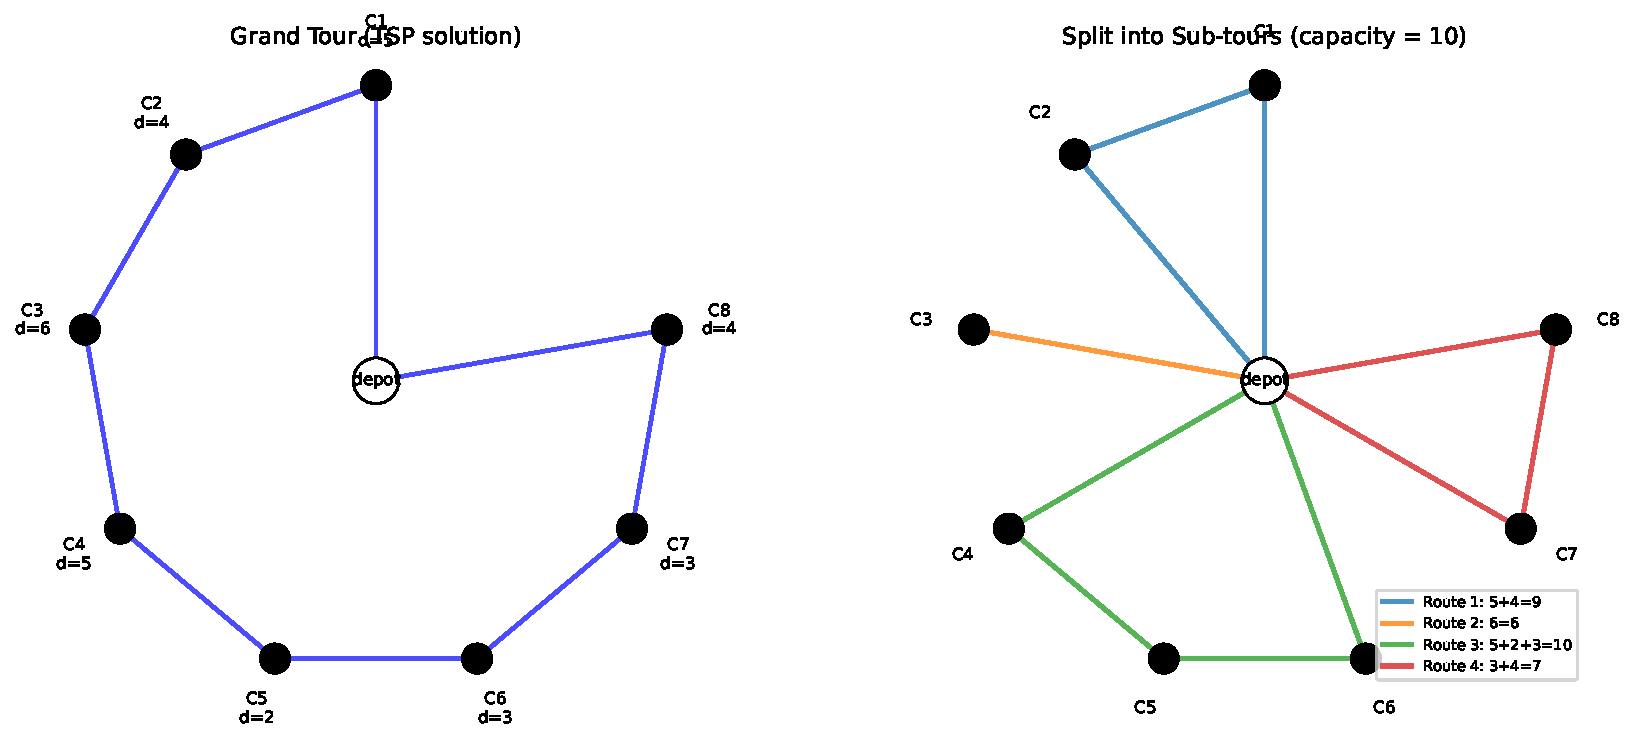
\includegraphics[width=0.75\textwidth]{fig_grand_tour_split.pdf}
  \end{center}

  The left panel shows the Grand Tour as a single TSP loop; the right panel
  shows the four sub-tours after splitting at capacity boundaries.

  \framebreak

  \begin{block}{Algorithm 6: CVRP from Grand Tour (Pseudocode)}
    \ttfamily\small
    \textbf{Procedure} \textsc{CvrpGrandTour}()\\
    \quad $\mathit{currentTour} \leftarrow [\,]$\\
    \quad $\mathit{currentDemand} \leftarrow 0$\\
    \quad \textbf{for} each visit $v$ in grand tour order \textbf{do}\\
    \quad\quad \textbf{if} $(\mathit{currentDemand} + v.\mathit{demand}) > Q$ \textbf{then}\\
    \quad\quad\quad $\mathit{result}.\mathrm{add}(\mathit{currentTour})$ \hfill\textit{// close current route}\\
    \quad\quad\quad $\mathit{currentTour} \leftarrow [\,]$\\
    \quad\quad\quad $\mathit{currentDemand} \leftarrow 0$\\
    \quad\quad $\mathit{currentTour}.\mathrm{append}(v)$\\
    \quad\quad $\mathit{currentDemand} \mathrel{+}= v.\mathit{demand}$\\
    \quad \textbf{return} $\mathit{result}$
  \end{block}

  \medskip
  The algorithm is a single pass through the sorted customer list.  Its
  \textbf{time complexity} is $O(n)$ once the Grand Tour order is known
  (finding the Grand Tour itself takes $O(n^2)$ for the Nearest-Neighbour
  TSP heuristic).  The algorithm is therefore very fast, but its quality
  depends heavily on the quality of the underlying TSP solution.

  \begin{alertblock}{Limitation of the Grand Tour}
    The Grand Tour splits customers according to the \emph{TSP order}, not
    geographic proximity under the capacity constraint.  Customers that are
    geographically close may end up in different routes simply because the
    TSP tour placed a capacity boundary between them.  This leads to solutions
    that use more distance than necessary.
  \end{alertblock}

\end{frame}

% ── Clarke-Wright ────────────────────────────────────────────
\begin{frame}[allowframebreaks]{The Clarke--Wright Savings Algorithm: Intuition}

  The Clarke--Wright algorithm (Clarke and Wright, 1964) attacks the CVRP
  from the opposite end.  Rather than starting with a TSP tour and splitting,
  it starts with the \emph{worst} possible solution and iteratively
  \emph{improves} it.

  \bigskip
  \textbf{Worst-case starting point.}  Suppose we send a separate vehicle to
  every customer --- $n$ vehicles, each making a single out-and-back trip from
  the depot to one customer.  This is obviously inefficient: every customer
  requires the full round-trip distance to the depot.  The total distance is
  $2 \sum_{i=1}^{n} \mathrm{dist}(d, c_i)$.

  \bigskip
  \textbf{The saving idea.}  If two customers $c_x$ and $c_y$ can be served
  by a single vehicle (i.e., their combined demand is $\leq Q$), we can
  replace the two separate trips $d \to c_x \to d$ and $d \to c_y \to d$
  with one merged trip $d \to c_x \to c_y \to d$.  The \textbf{saving} is:
  \[
    s(c_x, c_y) \;=\;
    \underbrace{\mathrm{dist}(d, c_x) + \mathrm{dist}(d, c_y)}_{\text{via depot}}
    \;-\;
    \underbrace{\mathrm{dist}(c_x, c_y)}_{\text{direct link}}
  \]

  The saving $s(c_x, c_y)$ is positive whenever the detour via the depot is
  longer than going directly from $c_x$ to $c_y$.  A large saving means we
  gain a lot by combining these two customers on one route.

  \framebreak

  \begin{center}
    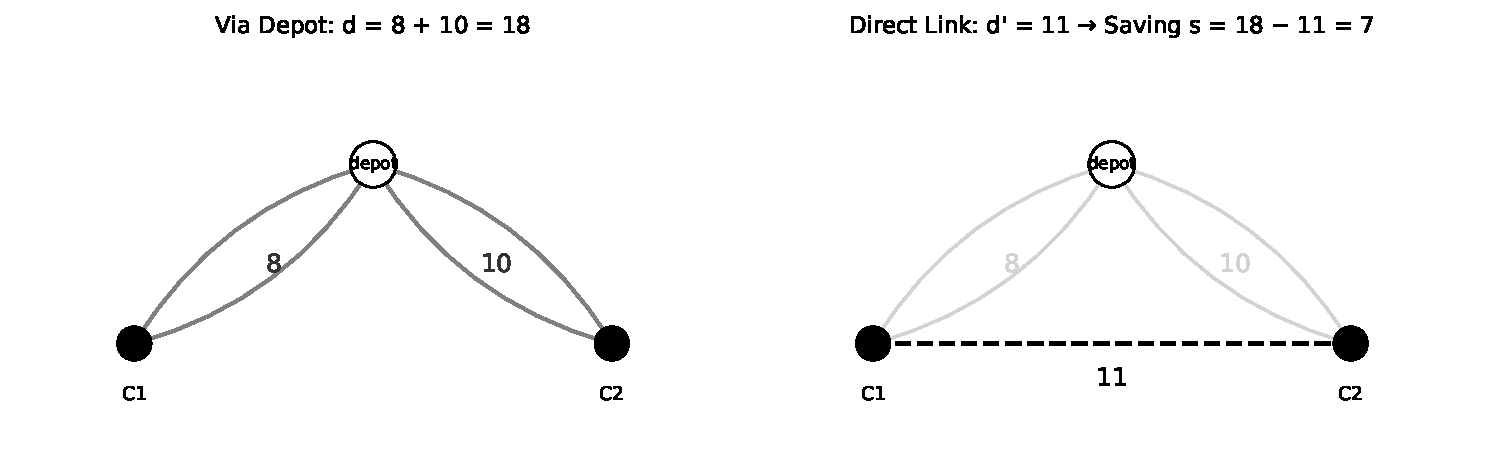
\includegraphics[width=0.82\textwidth]{fig_cw_savings.pdf}
  \end{center}

  \medskip
  \textbf{Reading the figure.}  The left panel shows two separate routes: each
  van goes to its customer and comes straight back.  The cost is
  $8 + 8 + 10 + 10 = 36$ distance units.  The right panel merges the two
  customers: one van goes to $C_1$, then directly to $C_2$, then returns to
  the depot.  The cost is $8 + 11 + 10 = 29$.  The saving is $36 - 29 = 7$.

  \framebreak

  \begin{block}{Savings Formula (Book Notation)}
    Let $d$ denote the depot.  For a pair of customers $c_x$ and $c_y$:
    \begin{enumerate}
      \item Compute the \textbf{via-depot distance}:
        \[
          d_{\text{via}} = \mathrm{dist}(c_x,\, d) + \mathrm{dist}(d,\, c_y)
        \]
      \item Compute the \textbf{direct distance}:
        \[
          d' = \mathrm{dist}(c_x,\, c_y)
        \]
      \item The \textbf{saving} is:
        \[
          s = d_{\text{via}} - d' = \bigl[\mathrm{dist}(c_x, d) + \mathrm{dist}(d, c_y)\bigr] - \mathrm{dist}(c_x, c_y)
        \]
    \end{enumerate}
  \end{block}

  \begin{alertblock}{How to Read This}
    A positive saving means it is cheaper to go from $c_x$ directly to $c_y$
    than to make two separate depot round-trips.  The larger the saving, the
    more we gain by combining these two customers.  If the saving is zero or
    negative, it is no cheaper (or more expensive) to combine them.
  \end{alertblock}

  \begin{exampleblock}{Numerical Example from the Book}
    $\mathrm{dist}(C_1, \text{depot}) = 8$, \quad
    $\mathrm{dist}(\text{depot}, C_2) = 10$, \quad
    $\mathrm{dist}(C_1, C_2) = 11$.

    \[
      d_{\text{via}} = 8 + 10 = 18, \qquad d' = 11, \qquad s = 18 - 11 = 7.
    \]

    Since $s = 7 > 0$, merging $C_1$ and $C_2$ on one route saves 7 units of
    distance.
  \end{exampleblock}

\end{frame}

% ── Clarke-Wright algorithm ──────────────────────────────────
\begin{frame}[allowframebreaks]{Clarke--Wright: The Full Algorithm}

  The complete Clarke--Wright procedure is:

  \begin{block}{Algorithm 7: Clarke--Wright Savings Algorithm}
    \begin{enumerate}
      \item \textbf{Initialise}: build one route per customer
        (the ``flower'' solution of Fig.~2.3 in the book).
      \item \textbf{Compute savings}: for every pair of customers $(c_x, c_y)$,
        compute $s = \mathrm{dist}(c_x, \text{depot}) + \mathrm{dist}(\text{depot}, c_y) - \mathrm{dist}(c_x, c_y)$.
        Store all pairs with $s > 0$.
      \item \textbf{Sort}: arrange the savings list in \emph{descending} order,
        so that the most beneficial merge is considered first.
      \item \textbf{Apply savings}: for each saving $(s, c_x, c_y)$ in order:
        \begin{enumerate}
          \item Find the route $r_x$ that contains $c_x$ at its \emph{end}.
          \item Find the route $r_y$ that contains $c_y$ at its \emph{start}.
          \item If $r_x \neq r_y$ \emph{and}
            the combined demand $d(r_x) + d(r_y) \leq Q$:
            \textbf{merge} $r_x$ and $r_y$ into a single route.
        \end{enumerate}
      \item \textbf{Return} the current solution (all remaining routes).
    \end{enumerate}
  \end{block}

  \framebreak

  \textbf{Why must $c_x$ be at the end and $c_y$ at the start of their routes?}
  Because the saving formula assumes the link goes $\ldots \to c_x \to c_y \to \ldots$,
  replacing the endings $\ldots \to c_x \to d$ and $d \to c_y \to \ldots$.
  If $c_x$ were in the middle of a route, inserting a direct link to $c_y$
  would require reversing part of the route, which changes the distance
  calculation.

  \bigskip
  The algorithm considers savings from largest to smallest.  This greedy
  ordering is not guaranteed to find the global optimum, but it ensures that
  the most beneficial merges are not blocked by suboptimal earlier decisions.

  \bigskip
  \begin{center}
    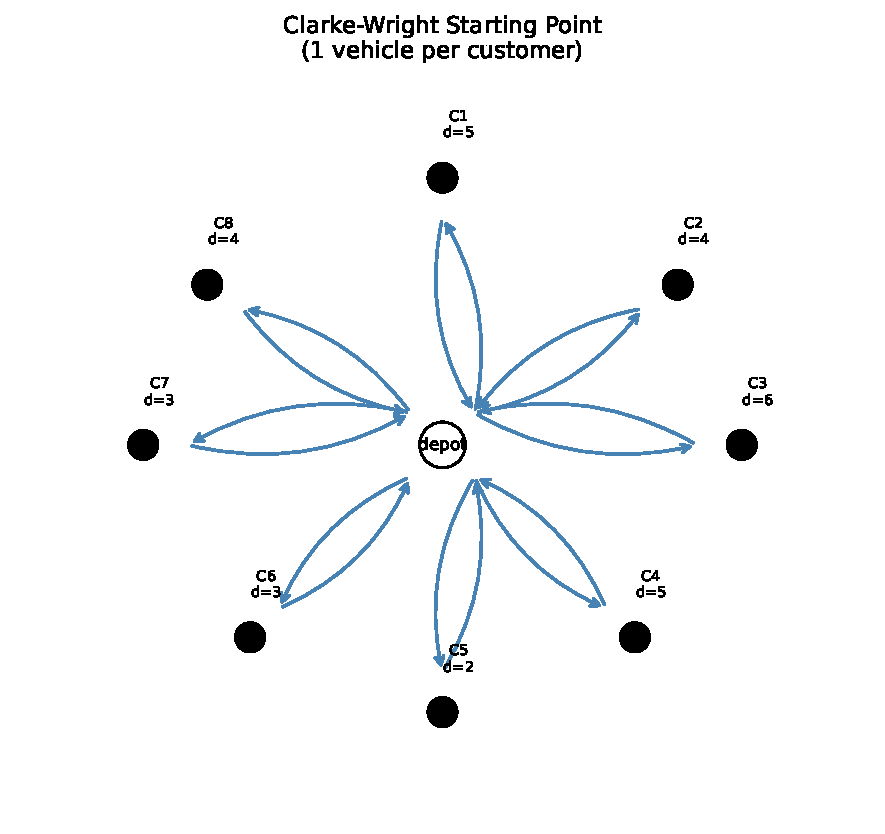
\includegraphics[width=0.38\textwidth]{fig_cw_start.pdf}
  \end{center}

  The starting point: each customer has its own round-trip route (the
  ``flower'' pattern).  The algorithm then merges pairs of petals into
  multi-customer routes.

  \framebreak

  \begin{block}{Formal Pseudocode (Algorithm 7 from the book)}
    \small
    \textbf{Procedure} \textsc{ClarkeWright}()\\
    \quad $savings \leftarrow []$ \\
    \quad $solution \leftarrow \textsc{BuildOnePerCust}()$ \\
    \quad \textbf{for} $v_x$ in problem, \textbf{for} $v_y$ in problem \textbf{do} \\
    \quad\quad $d \leftarrow \mathrm{dist}(v_x, \text{depot}) + \mathrm{dist}(\text{depot}, v_y)$ \\
    \quad\quad $d' \leftarrow \mathrm{dist}(v_x, v_y)$ \\
    \quad\quad $s \leftarrow d - d'$ \\
    \quad\quad \textbf{if} $s > 0$ \textbf{then} $savings.\text{add}(\text{Saving}(s, v_x, v_y))$ \\
    \quad $\textsc{Sort}(savings)$ \hfill // descending by $s$ \\
    \quad \textbf{for} saving $s$ in $savings$ \textbf{do} \\
    \quad\quad $r_x \leftarrow \textsc{route}(s.x)$;\quad $r_y \leftarrow \textsc{route}(s.y)$ \\
    \quad\quad \textbf{if} $r_x.\textit{last} == s.x$ \textbf{and} $r_y.\textit{first} == s.y$ \textbf{then} \\
    \quad\quad\quad \textbf{if} $d(r_x) + d(r_y) \leq \textit{cap}$ \textbf{then} \\
    \quad\quad\quad\quad $\textsc{merge}(r_x, r_y)$ \\
    \quad \textbf{return} $solution$
  \end{block}

  The inner double loop (lines 3--8) runs over all pairs of customers, giving
  $O(n^2)$ savings to compute.  Sorting is $O(n^2 \log n)$.  Applying savings
  is $O(n^2)$.  The overall time complexity is $\mathbf{O(n^2 \log n)}$,
  which is efficient for hundreds of customers but becomes slow for thousands.

\end{frame}

% ── CW flowchart ─────────────────────────────────────────────
\begin{frame}[allowframebreaks]{Clarke--Wright: Algorithm Flowchart}

  The flowchart below shows the full Clarke--Wright procedure graphically.
  Each diamond represents a decision point; each rectangle is an action step.
  The red arrows show the ``no'' branches (loop back to the next saving or
  skip the current saving).

  \begin{center}
    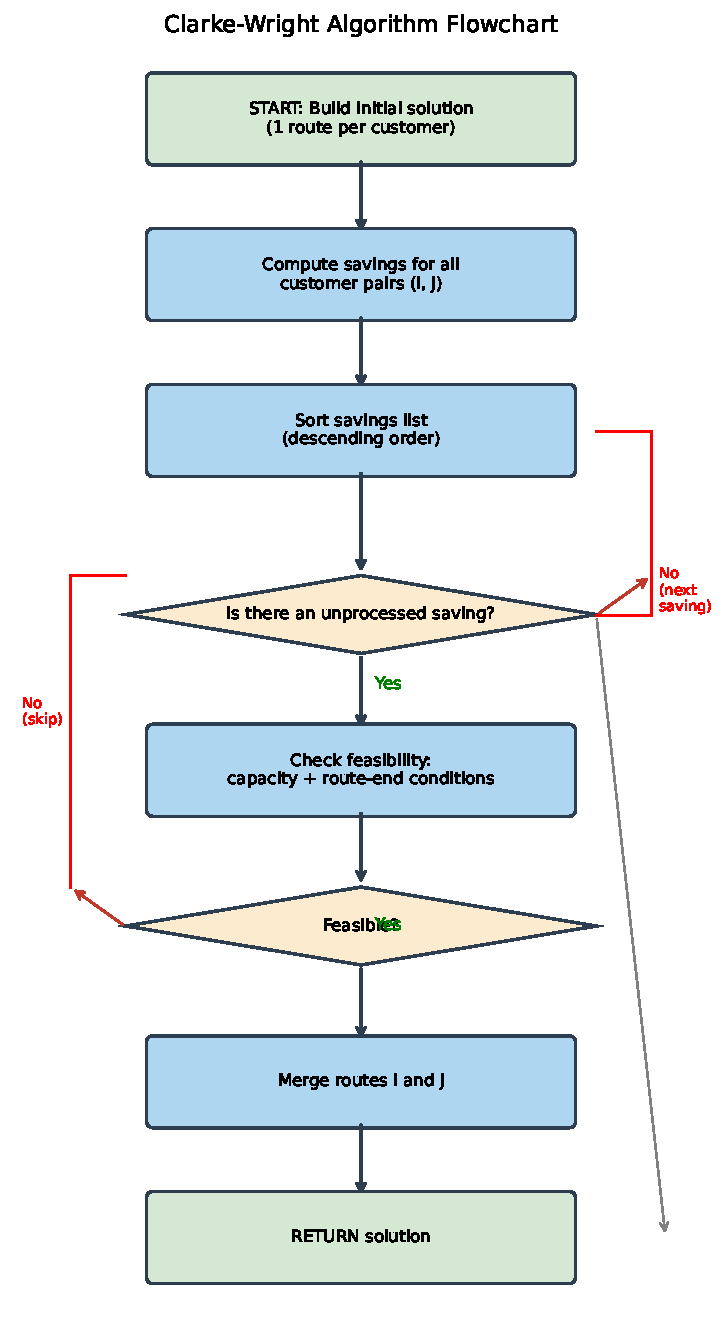
\includegraphics[width=0.36\textwidth]{fig_cw_flowchart.pdf}
  \end{center}

  \medskip
  The algorithm naturally terminates when the savings list is exhausted.
  Note that not all savings can be applied: a saving is skipped if either
  (a) the customers are already on the same route, (b) a customer is not at
  the required end/start position in its route, or (c) applying the saving
  would violate the capacity constraint.

\end{frame}

% ── CW worked example ────────────────────────────────────────
\begin{frame}[allowframebreaks]{Clarke--Wright: Step-by-Step Worked Example}

  Let us trace through the Clarke--Wright algorithm on the 8-customer instance.
  We use simplified distances for illustration.

  \bigskip
  \textbf{Initial solution:} 8 routes, one per customer.

  \medskip
  \textbf{Sample savings (sorted largest-first):}

  \begin{center}
    \small
    \begin{tabular}{ccccc}
      \toprule
      Rank & Pair $(c_x, c_y)$ & $d_{\text{via depot}}$ & $d'$ (direct) & Saving $s$ \\
      \midrule
      1 & $(C_1, C_2)$ & 18 & 11 & 7 \\
      2 & $(C_4, C_5)$ & 17 & 10 & 7 \\
      3 & $(C_3, C_4)$ & 20 & 14 & 6 \\
      4 & $(C_6, C_7)$ & 16 & 11 & 5 \\
      5 & $(C_2, C_3)$ & 19 & 15 & 4 \\
      \bottomrule
    \end{tabular}
  \end{center}

  \framebreak

  \textbf{Applying savings in order:}

  \medskip
  \begin{enumerate}
    \item \textbf{Saving 1} $(C_1, C_2)$, $s=7$: Both are at the end/start of
      their individual routes.  Combined demand $5+4=9 \leq 10$.
      \textbf{Merge}: $d \to C_1 \to C_2 \to d$ (load~=~9).
    \item \textbf{Saving 2} $(C_4, C_5)$, $s=7$: Both are at the end/start of
      their routes.  Combined demand $5+2=7 \leq 10$.
      \textbf{Merge}: $d \to C_4 \to C_5 \to d$ (load~=~7).
    \item \textbf{Saving 3} $(C_3, C_4)$, $s=6$: $C_3$ is at the end of its
      route and $C_4$ is at the \emph{start} of $d \to C_4 \to C_5 \to d$.
      Combined demand $6 + 7 = 13 > 10$.  \textbf{Skip} (capacity violated).
    \item \textbf{Saving 4} $(C_6, C_7)$, $s=5$: Both at end/start.
      Combined $3+3=6 \leq 10$.
      \textbf{Merge}: $d \to C_6 \to C_7 \to d$ (load~=~6).
    \item \textbf{(Continue)} \ldots\ Eventually $C_5$ might be merged with $C_6$
      depending on route endpoint positions.
  \end{enumerate}

  \medskip
  Final solution may end up with 4 routes similar to: $\{C_1,C_2\}$,
  $\{C_3\}$, $\{C_4,C_5\}$, $\{C_6,C_7,C_8\}$ (exact result depends on
  all pairwise distances).

  \begin{alertblock}{Key Insight}
    The Clarke--Wright algorithm is \emph{greedy}: it always applies the
    largest available saving that is feasible.  This does not guarantee an
    optimal solution, but in practice the greedy ordering works well because
    it prioritises the most geographically natural route merges first.
  \end{alertblock}

\end{frame}

% ============================================================
%  SECTION 2.3 – IMPLEMENTATION
% ============================================================
\section{2.3 Implementation}

\begin{frame}[allowframebreaks]{Software Architecture}

  The book's implementation uses Java with an object-oriented class hierarchy
  that cleanly separates the \emph{problem} from the \emph{solver}.  This
  design pattern --- the Strategy pattern --- is important because it allows
  different solvers to be swapped in without changing the problem class.

  \begin{center}
    
\includegraphics[width=0.82\textwidth]{fig_class_diagram.pdf}
  \end{center}

  \framebreak

  The architecture has three layers:

  \begin{description}
    \item[\texttt{CVRPProblem}] Stores the problem data: the list of
      \texttt{VRPVisit} objects (customers), the vehicle capacity, and the
      current best solution (as a list of lists of visits).  Provides methods
      to compute solution distance and vehicle count.
    \item[\texttt{VRPSolver} (abstract)] Defines the interface that all
      CVRP solvers must implement: \texttt{solve()} and
      \texttt{setProblem(CVRPProblem)}.  This is an abstract class --- it
      cannot be instantiated directly.
    \item[\texttt{GrandTour}, \texttt{ClarkeWright}] Concrete solver classes
      that extend \texttt{VRPSolver} and implement the \texttt{solve()} method
      with their respective algorithms.
    \item[\texttt{VRPVisit}] Extends \texttt{Visit} (from Chapter~1) with an
      additional \texttt{demand} field.
    \item[\texttt{VRPProblemFactory}] A factory class that reads a problem
      instance from a file and returns a \texttt{CVRPProblem} object.
  \end{description}

  \medskip
  This separation ensures that adding a new solver (e.g., a genetic algorithm)
  in a later chapter only requires writing a new class that extends
  \texttt{VRPSolver} --- the rest of the code is unchanged.

\end{frame}

% ── Python Grand Tour ────────────────────────────────────────
\begin{frame}[fragile]{Python: Grand Tour Implementation}

  The following Python code implements the Grand Tour algorithm.  It mirrors
  the Java \texttt{GrandTour.solve()} method from Listing~2.1 in the book,
  translated into idiomatic Python.

\begin{lstlisting}[caption={Grand Tour CVRP solver (Python)}]
from dataclasses import dataclass
from typing import List
import math

@dataclass
class VRPVisit:
    name: str
    lat:  float
    lon:  float
    demand: int

    def distance(self, other: 'VRPVisit') -> float:
        return math.hypot(self.lat - other.lat, self.lon - other.lon)

class GrandTour:
    """
    Build a CVRP solution from a Grand Tour.
    Assumes `problem.solution` has already been set to a TSP tour
    (flat list of VRPVisit) by a TSP solver such as NearestNeighbour.
    """
    def __init__(self, problem):
        self.problem = problem   # CVRPProblem object

    def solve(self) -> List[List[VRPVisit]]:
        solution      = []           # list of completed routes
        current_route = []           # visits on the current route
        current_demand = 0           # total demand on current route

        # Walk through the pre-computed TSP tour
        for visit in self.problem.get_tsp_solution():
            vrp_visit = visit  # VRPVisit

            # If adding this customer would exceed capacity, close route
            if current_demand + vrp_visit.demand > self.problem.capacity:
                solution.append(current_route)   # save completed route
                current_route  = []              # start new route
                current_demand = 0

            current_route.append(vrp_visit)
            current_demand += vrp_visit.demand

        solution.append(current_route)   # add the final route
        self.problem.solution = solution
        return solution
\end{lstlisting}

\end{frame}

% ── Python Clarke-Wright main ────────────────────────────────
\begin{frame}[fragile]{Python: Clarke--Wright --- Main Outline}

  The Clarke--Wright solver is built from three methods.  Here is the main
  \texttt{solve()} method (corresponding to Listing~2.3 in the book):

\begin{lstlisting}[caption={Clarke--Wright main \texttt{solve()} method}]
from dataclasses import dataclass, field
from typing import List, Optional
import math, itertools

@dataclass(order=True)
class Saving:
    saving: float             # sort key (descending after negation)
    x: VRPVisit = field(compare=False)
    y: VRPVisit = field(compare=False)

class ClarkeWright:
    def __init__(self, problem):
        self.problem = problem

    def solve(self) -> List[List[VRPVisit]]:
        # Step 1: Create initial solution (1 route per customer)
        solution = [[v] for v in self.problem.visits]

        # Step 2: Find all savings
        savings = self._find_savings()

        # Step 3: Sort savings largest-first
        savings.sort(key=lambda s: -s.saving)

        # Step 4: Apply feasible savings
        self._apply_savings(solution, savings)

        # Step 5: Verify and store
        self._check_solution(solution)
        self.problem.solution = solution
        return solution
\end{lstlisting}

  Notice the four numbered comments --- they map directly onto the four
  conceptual phases of the Clarke--Wright algorithm.

\end{frame}

% ── Python find savings ──────────────────────────────────────
\begin{frame}[fragile]{Python: Clarke--Wright --- Finding Savings}

  The \texttt{\_find\_savings()} method iterates over every ordered pair of
  customers and computes the saving for each pair (Listing~2.4 in the book):

\begin{lstlisting}[caption={Clarke--Wright: computing all pairwise savings}]
    def _find_savings(self) -> List[Saving]:
        savings = []
        depot = self.problem.depot    # the depot VRPVisit object

        # Consider every ordered pair (x, y) of customers
        for x_idx, x in enumerate(self.problem.visits):
            for y_idx, y in enumerate(self.problem.visits):
                if x_idx == y_idx:
                    continue          # skip a customer paired with itself

                # Cost via depot: depot-to-x, x-to-depot, depot-to-y, y-to-depot
                # Saving = (x->depot + depot->y) - (x->y)
                cost_via_depot = (x.distance(depot)
                                  + depot.distance(y))
                direct_dist    = x.distance(y)
                s              = cost_via_depot - direct_dist

                savings.append(Saving(saving=s, x=x, y=y))

        return savings
\end{lstlisting}

  \medskip
  The time complexity of this method is $O(n^2)$ because it examines all
  $n(n-1)$ ordered pairs.  For $n=100$ customers that is 9,900 savings --- a
  trivial computation for modern hardware.

\end{frame}

% ── Python apply savings ─────────────────────────────────────
\begin{frame}[fragile]{Python: Clarke--Wright --- Applying Savings}

  The \texttt{\_apply\_savings()} method tries to merge routes, checking the
  feasibility conditions (Listing~2.5 in the book):

\begin{lstlisting}[caption={Clarke--Wright: applying savings to merge routes}]
    def _apply_savings(self, solution, savings):
        for s in savings:
            route_x = route_y = None

            # Find the routes containing s.x (as last element)
            #                          and s.y (as first element)
            for route in solution:
                if route and route[-1] == s.x:   # s.x at END of route
                    route_x = route
                if route and route[0]  == s.y:   # s.y at START of route
                    route_y = route

            # Merge only if both are found and belong to DIFFERENT routes
            if route_x is not None and route_y is not None:
                if route_x is not route_y:        # different routes
                    combined_demand = (
                        sum(v.demand for v in route_x)
                        + sum(v.demand for v in route_y)
                    )
                    if combined_demand <= self.problem.capacity:
                        # Merge: append route_y onto route_x
                        route_x.extend(route_y)
                        solution.remove(route_y)

            # Also try the reverse direction (y->x)
            # ... (similar logic with route_x[-1]==s.y, route_y[0]==s.x)
\end{lstlisting}

\end{frame}

% ── Python complete example ──────────────────────────────────
\begin{frame}[fragile]{Python: Running the CVRP Solvers}

  The following snippet shows how to set up a CVRP problem and run both
  solvers --- mirroring the book's \texttt{main()} / Listing~2.2:

\begin{lstlisting}[caption={Using the Grand Tour and Clarke--Wright solvers}]
# Build a small test instance (8 customers, capacity 10)
visits = [
    VRPVisit('C1',  0.0,  2.5, 5),
    VRPVisit('C2',  2.2,  1.5, 4),
    VRPVisit('C3',  2.8,  0.0, 6),
    VRPVisit('C4',  1.8, -1.8, 5),
    VRPVisit('C5',  0.0, -2.5, 2),
    VRPVisit('C6', -1.8, -1.8, 3),
    VRPVisit('C7', -2.8,  0.0, 3),
    VRPVisit('C8', -2.2,  1.5, 4),
]
depot = VRPVisit('depot', 0.0, 0.0, 0)

problem = CVRPProblem(visits=visits, depot=depot, capacity=10)

# --- Grand Tour ---
nn_solver = NearestNeighbourSolver(problem)   # solve TSP first
nn_solver.solve()
gt_solver = GrandTour(problem)
gt_solution = gt_solver.solve()
print(f"Grand Tour:      distance={problem.get_distance():.1f}, "
      f"vehicles={len(gt_solution)}")

# --- Clarke-Wright ---
cw_solver = ClarkeWright(problem)
cw_solution = cw_solver.solve()
print(f"Clarke-Wright:   distance={problem.get_distance():.1f}, "
      f"vehicles={len(cw_solution)}")
\end{lstlisting}

\end{frame}

% ============================================================
%  SECTION 2.4 – RESULTS
% ============================================================
\section{2.4 Results}

\begin{frame}[allowframebreaks]{Experimental Setup}

  To evaluate the two heuristics, they are run on all 60 Augerat benchmark
  instances.  For each instance, the following quantities are recorded:
  \begin{itemize}
    \item The \textbf{total distance} of the solution produced.
    \item The \textbf{number of vehicles} used.
  \end{itemize}
  These are then compared against the branch-and-cut optimal (or best-known)
  results published by Augerat (1995).

  \bigskip
  For the Grand Tour heuristic, the Nearest-Neighbour TSP solver is used to
  generate the initial tour (as in Listing~2.2 of the book).

  \bigskip
  \begin{block}{Performance Metric}
    The key metric is the \textbf{percentage excess above best known}:
    \[
      \text{excess}(\%) = \frac{\text{heuristic distance} - \text{best-known distance}}
                               {\text{best-known distance}} \times 100
    \]
    A value of 0\% means the heuristic matched the best-known solution exactly.
    A value of 25\% means the heuristic's routes are 25\% longer than optimal.
  \end{block}

\end{frame}

\begin{frame}[allowframebreaks]{Results: Selected Instances from Table 2.1 (Set A)}

  The table below shows a selection of Set~A results.  The ``B\&C'' column
  gives the branch-and-cut reference; the other columns give the Grand Tour
  and Clarke--Wright results.  Problem names have the form
  \texttt{A-n\emph{X}-k\emph{Y}}, meaning Set~A, $n=X$ customers, $k=Y$
  vehicles in the best solution.

  \medskip
  \begin{center}
    \small
    \begin{tabular}{lrr@{\quad}rr@{\quad}rr}
      \toprule
      Problem & B\&C dist & B\&C veh
              & GT dist & GT veh
              & C-W dist & C-W veh \\
      \midrule
      A-n32-k5  &  784 & 5 & 1023.9 & 5 &  810.8 & 5 \\
      A-n33-k5  &  661 & 5 &  777.8 & 5 &  712.0 & 5 \\
      A-n33-k6  &  742 & 6 &  880.5 & 6 &  776.3 & 7 \\
      A-n36-k5  &  799 & 5 &  975.6 & 5 &  834.4 & 5 \\
      A-n37-k5  &  669 & 5 &  968.2 & 5 &  707.3 & 5 \\
      A-n39-k5  &  822 & 5 & 1061.0 & 5 &  894.7 & 5 \\
      A-n45-k6  &  944 & 6 & 1160.7 & 6 & 1013.3 & 7 \\
      A-n53-k7  & 1010 & 7 & 1208.4 & 7 & 1097.6 & 7 \\
      \bottomrule
    \end{tabular}
  \end{center}

  \medskip
  Looking at A-n32-k5: the branch-and-cut optimum is 784; the Grand Tour
  produces 1023.9 (31\% above optimum); Clarke--Wright produces 810.8 (only
  3.4\% above).  Clarke--Wright is clearly the better heuristic for this
  instance.

  \framebreak

  \begin{center}
    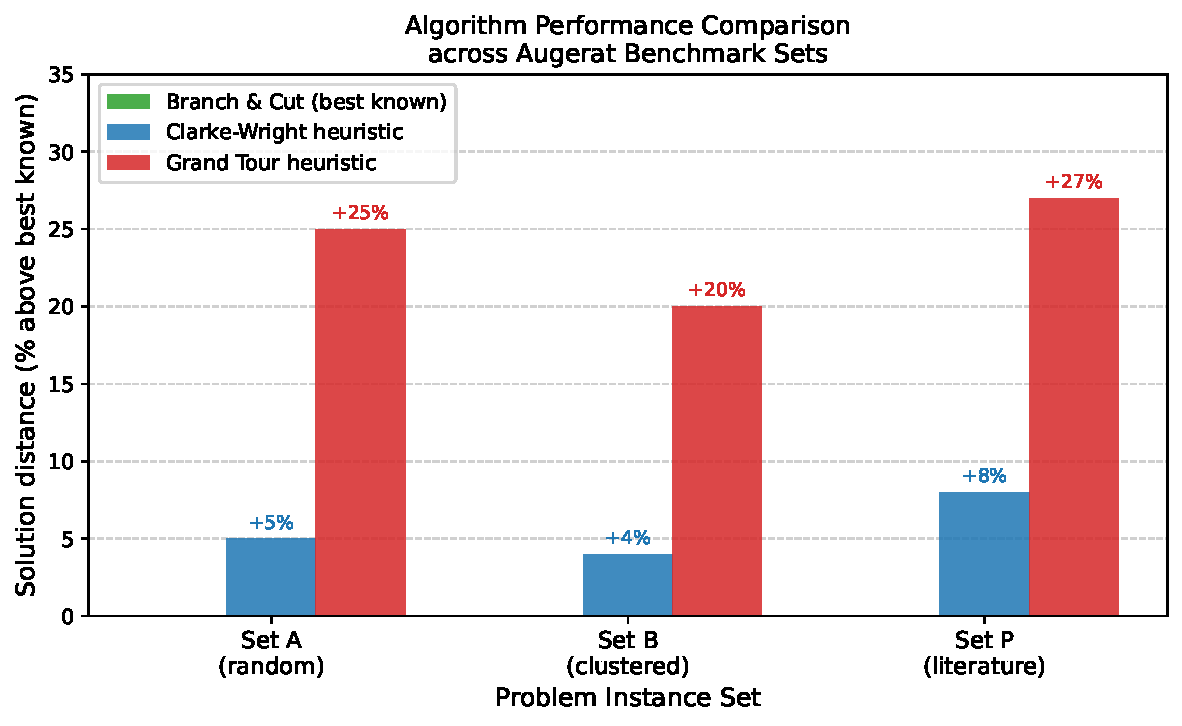
\includegraphics[width=0.72\textwidth]{fig_benchmark_comparison.pdf}
  \end{center}

  \medskip
  The bar chart aggregates results across all three Augerat sets.  The key
  observation is that Clarke--Wright is substantially better than Grand Tour:
  it produces solutions only 5--8\% longer than the best known, while Grand
  Tour is 20--27\% longer.  However, \emph{both} heuristics are still
  noticeably worse than branch and cut --- indicating that more sophisticated
  optimisation is needed.

\end{frame}

\begin{frame}[allowframebreaks]{Results: Solution Visualisation}

  The figure below (from the book's Fig.~2.5) shows the P-n20-k2 problem
  instance solved in three ways.  Examining these visual solutions helps
  understand \emph{why} the Grand Tour performs poorly.

  \begin{center}
    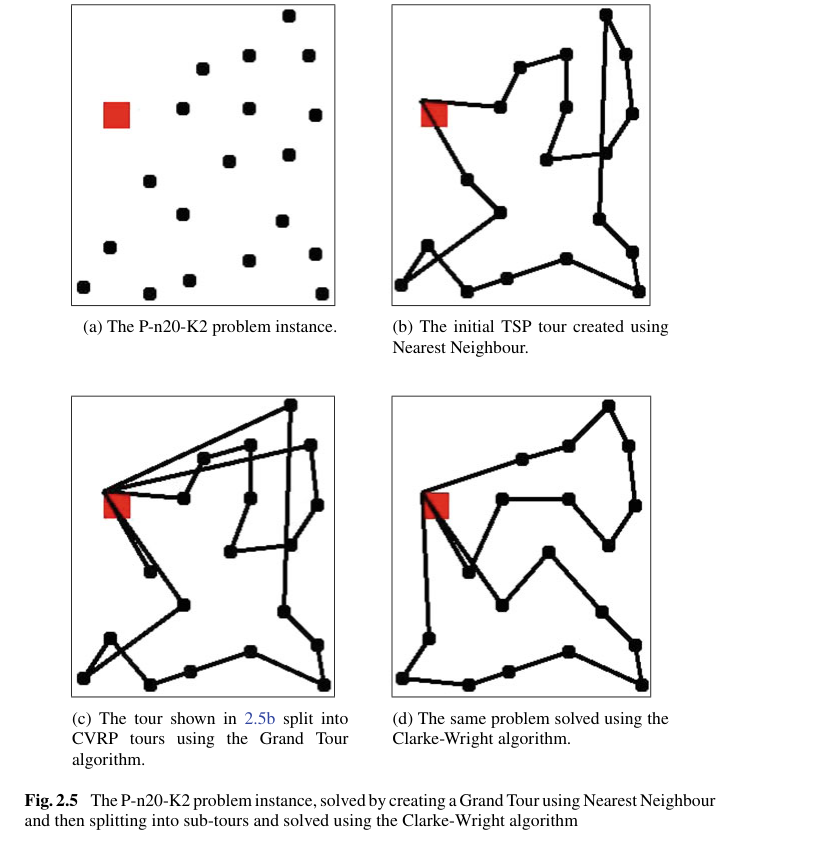
\includegraphics[width=0.88\textwidth]{fig_solution_comparison.png}
  \end{center}

  \medskip
  \textbf{Reading the figure (left to right):}

  \begin{enumerate}
    \item \textbf{(a) Problem instance}: the raw customer locations and depot.
    \item \textbf{(b) TSP tour (Nearest Neighbour)}: the initial Grand Tour
      threads through all customers.  The Nearest-Neighbour heuristic produces
      a tour that avoids obvious long jumps but is not globally optimal.
    \item \textbf{(c) Grand Tour split}: the TSP tour is cut at capacity
      boundaries, producing 3 CVRP routes.  Notice that some routes contain
      geographically spread-out customers because the capacity boundary falls
      in an inconvenient place.
    \item \textbf{(d) Clarke--Wright}: the Clarke--Wright algorithm produces 2
      cleaner routes that match the best-known solution, grouping geographically
      close customers together.
  \end{enumerate}

  \medskip
  The Grand Tour retains the ``imperfections'' of the Nearest-Neighbour TSP
  heuristic --- including the loop in the lower-left corner --- because the
  splitting step cannot re-order customers within a route.

\end{frame}

\begin{frame}[allowframebreaks]{Why Clarke--Wright Outperforms Grand Tour}

  The performance gap between Clarke--Wright and Grand Tour has a clear
  structural explanation:

  \bigskip
  The Grand Tour heuristic is \textbf{sequential}: it first optimises for
  distance (via the TSP solver) \emph{ignoring} the capacity constraint, then
  enforces the constraint by cutting the tour.  The cuts are made mechanically
  at capacity boundaries without regard for geography --- a cut might separate
  two customers who are close to each other.

  \bigskip
  Clarke--Wright is \textbf{capacity-aware from the start}: it begins with
  the capacity constraints fully respected (one vehicle per customer) and
  merges routes only when doing so is both feasible and beneficial.  The
  savings criterion naturally groups geographically close customers together,
  because nearby customers have small direct distances and therefore large
  savings.

  \begin{alertblock}{The Core Insight}
    The Clarke--Wright savings criterion is a proxy for geographic proximity:
    customers that are close to each other (small $d'$) and far from the depot
    (large $d_{\text{via}}$) produce large savings.  So the algorithm
    naturally groups nearby customers on the same route --- exactly what a
    good delivery plan should do.
  \end{alertblock}

\end{frame}

% ============================================================
%  SECTION 2.5 – CONCLUSIONS
% ============================================================
\section{2.5 Conclusions}

\begin{frame}[allowframebreaks]{Conclusions and Limitations}

  This chapter has introduced the CVRP and two classic heuristic solvers.
  The Grand Tour and Clarke--Wright algorithms both produce \emph{feasible}
  solutions quickly --- but how good are they in practice?

  \bigskip
  \textbf{Grand Tour Assessment:}
  \begin{itemize}
    \item Simple to implement: one loop over a sorted list.
    \item Very fast: $O(n)$ after the TSP tour is computed.
    \item Poor quality: 20--27\% above optimal on average.
    \item The quality depends entirely on the TSP solver --- if the Grand Tour
      has many long edges, the CVRP solution will also have long routes.
    \item Cannot group customers based on demand; the order is fixed by the TSP.
  \end{itemize}

  \bigskip
  \textbf{Clarke--Wright Assessment:}
  \begin{itemize}
    \item More complex to implement, but still straightforward.
    \item Time complexity $O(n^2 \log n)$: slower than Grand Tour but efficient
      for hundreds of customers.
    \item Much better quality: 5--8\% above optimal on average.
    \item Greedy strategy is not guaranteed to be optimal; it can get stuck
      in local optima.
  \end{itemize}

  \framebreak

  \textbf{The fundamental limitation of both heuristics} is that they are
  \emph{construction} methods: they build a solution in one pass and cannot
  escape from a poor choice made early on.  Neither algorithm includes a
  mechanism to \emph{improve} an existing solution after it has been built.

  \bigskip
  \begin{block}{What Comes Next?}
    To achieve results comparable with branch-and-cut, we need a more powerful
    technique.  The key insight is that we require two capabilities:
    \begin{enumerate}
      \item A way to \textbf{escape local optima} --- to accept temporarily
        worse solutions in order to later find better ones.
      \item A way to \textbf{leverage domain knowledge} --- for example,
        by focusing on geographically natural customer groupings.
    \end{enumerate}
    The subsequent chapters introduce nature-inspired metaheuristics (genetic
    algorithms, simulated annealing, ant colony optimisation) that address
    both of these needs and consistently outperform Clarke--Wright.
  \end{block}

  \begin{alertblock}{Summary of Chapter 2}
    The CVRP is NP-hard and requires either exponential-time exact methods
    (branch and cut) or fast heuristics.  Clarke--Wright (1964) remains one
    of the best simple heuristics: easy to implement, $O(n^2 \log n)$,
    and typically 5--8\% above optimal.  It serves as the baseline that
    all more sophisticated solvers in this book aim to beat.
  \end{alertblock}

\end{frame}

% ── Final summary ────────────────────────────────────────────
\begin{frame}[allowframebreaks]{Chapter Summary: Key Formulas and Concepts}

  \begin{block}{CVRP Capacity Constraint}
    For every route $r_j$:
    \[
      \sum_{i \in r_j} \delta_i \;\leq\; Q
    \]
    Each $\delta_i$ (delta) is the demand of customer $i$; $Q$ is the vehicle
    capacity.  No route can carry more than $Q$ units.
  \end{block}

  \begin{block}{Minimum Vehicles Lower Bound}
    \[
      k_{\min} = \left\lceil \frac{\sum_{i=1}^{n} \delta_i}{Q} \right\rceil
    \]
    The total demand divided by capacity, rounded up.  This is a theoretical
    minimum; the actual solution may require more vehicles.
  \end{block}

  \begin{block}{Clarke--Wright Saving}
    \[
      s(c_x, c_y) = \mathrm{dist}(c_x, d) + \mathrm{dist}(d, c_y) - \mathrm{dist}(c_x, c_y)
    \]
    A positive saving means it is cheaper to link $c_x$ directly to $c_y$
    than to route both via the depot separately.
  \end{block}

  \framebreak

  \begin{block}{Algorithm Complexity Summary}
    \begin{center}
      \begin{tabular}{lll}
        \toprule
        Algorithm & Time complexity & Solution quality \\
        \midrule
        Grand Tour    & $O(n^2)$ (with NN TSP)   & 20--27\% above optimum \\
        Clarke--Wright & $O(n^2 \log n)$          & 5--8\% above optimum \\
        Branch and cut & Exponential (worst case) & Optimal \\
        \bottomrule
      \end{tabular}
    \end{center}
  \end{block}

  \begin{block}{Augerat Benchmark Sets}
    \begin{itemize}
      \item \textbf{Set A}: 30 instances, random customer placement,
        $n = 31$--80 customers.
      \item \textbf{Set B}: 20 instances, clustered customer placement,
        $n = 31$--78.
      \item \textbf{Set P}: 24 instances, literature-based instances,
        $n = 16$--101.
    \end{itemize}
    All instances have known optimal or best-known solutions.  The total
    collection of 60 problems provides a comprehensive evaluation platform.
  \end{block}

  \begin{alertblock}{Bottom Line}
    Clarke--Wright is fast, simple, and produces solutions that are practically
    useful (within 8\% of optimal on typical instances).  It is the standard
    baseline against which all more advanced CVRP solvers are measured.
    Nature-inspired methods introduced in later chapters consistently achieve
    2--4\% above optimal --- roughly halving the error of Clarke--Wright.
  \end{alertblock}

\end{frame}

% ── References ───────────────────────────────────────────────
\begin{frame}[allowframebreaks]{References}

  \begin{itemize}
    \item Augerat, P.\ (1995). \textit{Approche poly\`edrale du probl\`eme de
      tourn\'ees de v\'ehicules} [Polyhedral approach of the vehicle routing
      problem]. PhD thesis, Grenoble Institute of Technology, France.

    \item Augerat, P.\ (2014a,b,c). VRP-REP: Augerat 1995 Sets A, B, P.
      \texttt{http://www.vrp-rep.org/datasets/}

    \item Clarke, G., and Wright, J.W.\ (1964). Scheduling of vehicles from a
      central depot to a number of delivery points. \textit{Operations Research},
      12(4), 568--581.

    \item Dantzig, G.B., and Ramser, J.H.\ (1959). The truck dispatching
      problem. \textit{Management Science}, 6(1), 80--91.

    \item Gendreau, M., et al.\ (2008). Metaheuristics for the vehicle routing
      problem and its extensions: a categorized bibliography. In
      \textit{The Vehicle Routing Problem: Latest Advances and New Challenges}.
      Springer.

    \item Laporte, G.T.\ (2013). Vehicle routing: historical perspective and
      recent contributions. \textit{EURO Journal on Transportation and
      Logistics}, 2(1--2).

    \item Solomon, M.M.\ (1987). Algorithms for the vehicle routing and
      scheduling problems with time window constraints. \textit{Operations
      Research}, 35(2), 254--265.
  \end{itemize}

\end{frame}

\end{document}
